\chapter{System Model}
\label{ch:architecture}

如果想在latex裡面插入表格, 可以搜尋latex table generator, 有很多線上網站可以參考. 我個人都是使用線上網站去產生大致的語法, 然後再根據個人喜好去做微調, wikibook有很多資料可以參考, 網址在這邊: https://en.wikibooks.org/wiki/LaTeX/Tables

如果要引用表格, 記得在table裡加上label的語法, 然後就可以呼叫 Tab~\ref{tab1}, 寫中文的就是表~\ref{tab1}. 通常Table的caption是寫在表格的上面, 圖片則是放在下面.

\begin{table}[!ht]
    \centering
    \caption{This is a table.}
    \label{tab1}
    \begin{tabular}{|l|l|l|l|}
    \hline
        A & 1 & 4 & 7 \\ \hline
        B & 2 & 5 & 8 \\ \hline
        C & 3 & 6 & 9 \\ \hline
    \end{tabular}
\end{table}

後來在圖書館的``2022 研究攻略營 論文寫作實戰技巧(顏安孜老師)''看到另一種作法,網址: http://bit.ly/3yE06Hx

裡面的講義有提到Excel2LaTeX,細節可以去看圖書館的連結,裡面有放講義,下方是顏安孜老師的講義截圖

\begin{figure}[htb]
	\centering
	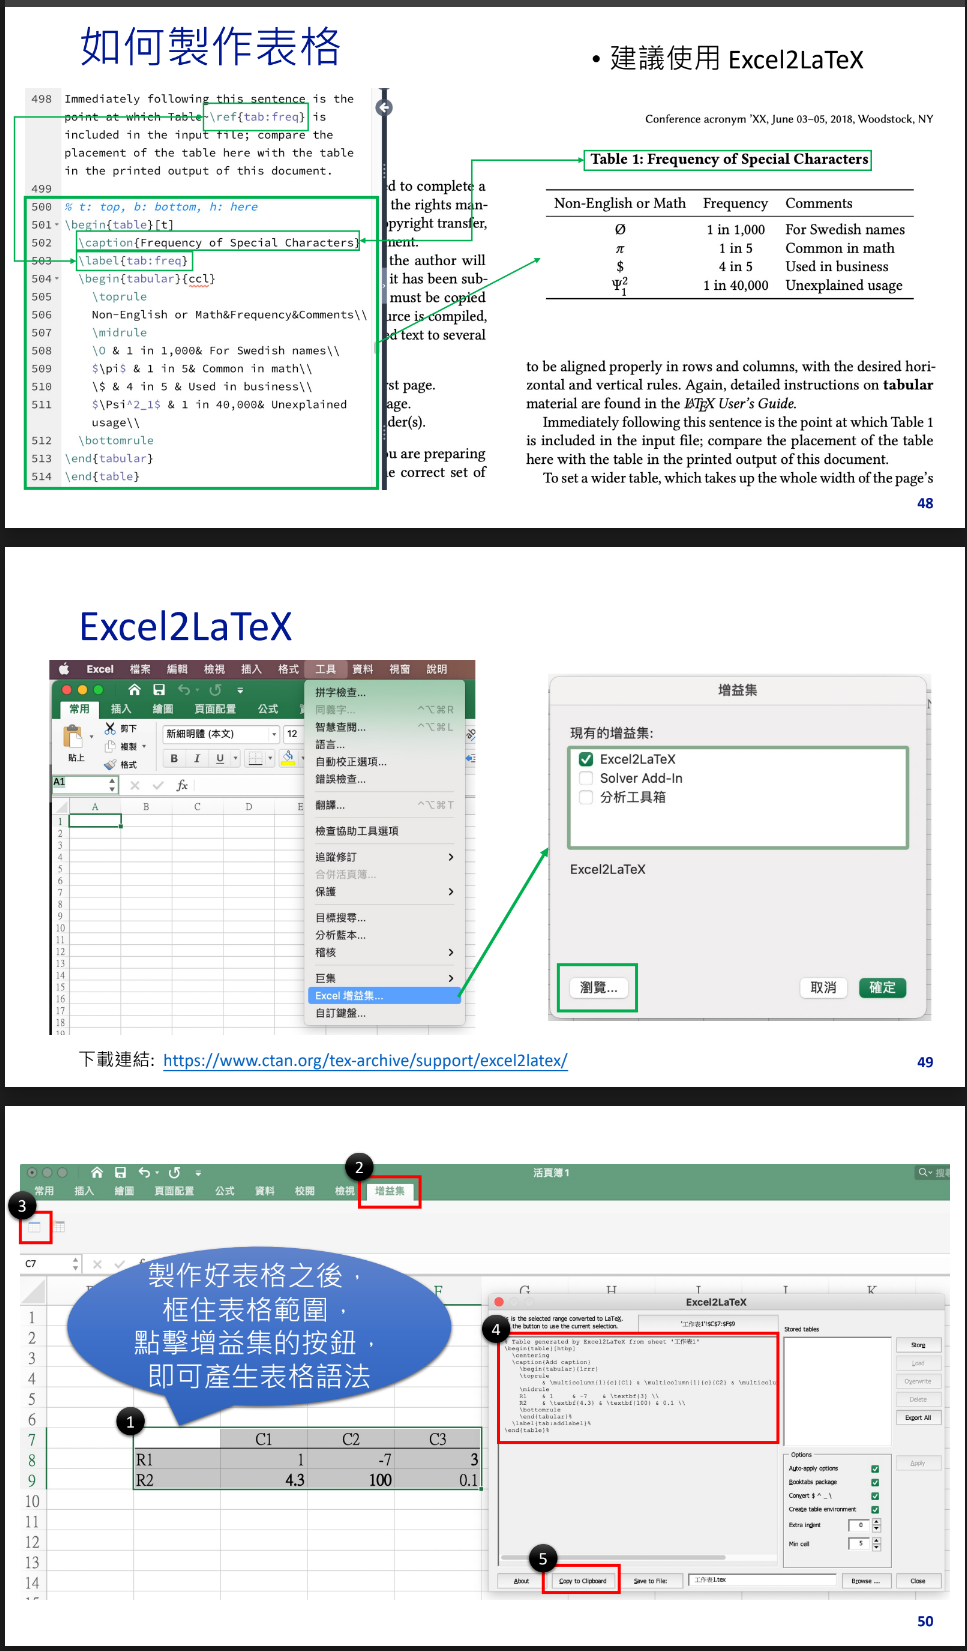
\includegraphics[width=0.8\textwidth]{img/excel2latex.png}
	\caption{Excel2LaTeX.}
	\label{fig:excel2latex}
\end{figure}

